\section{Ambiente di Lavoro}

\subsection{Coordinamento}
\subsubsection{Software di Versionamento}

Il software scelto per la gestione del versionamento, dopo accurata analisi di altri prodotti (come SVN o Mercurial), è \glossario{GitHub}. I motivi principali della scelta sono:
\begin{itemize}
\item \textbf{Interfaccia Grafica}: a differenza di \glossario{Git} che prevede un utilizzo unicamente da linea di comando, \glossario{GitHub} fornisce un'interfaccia grafica molto ben fatta e comprensibile per tutti i membri del gruppo; inoltre è possibile consultare online tutti i file inseriti nel \glossario{repository}, senza fare una copia locale, ed è permesso controllare le differenze tra la versione ed un'altra di un singolo file, in modo da capire le differenze ed eventualmente risolvere i conflitti che si possono venire a creare;
\item \textbf{Flessibilità}: \glossario{GitHub} è un \glossario{repository} distribuito che prevede la possibilità di \glossario{commit} e \glossario{revert} locali;
\item \textbf{Servizi aggiuntivi}: \glossario{GitHub} provvede a fornire, ad esempio, servizi di controllo accessi e \glossario{bug tracking}, molto utili per la gestione efficiente del progetto;
\item \textbf{Esperienza del Gruppo}: \glossario{GitHub} è già stato usato da alcuni componenti del gruppo \GroupName{}.
\end{itemize}

\subsubsection{Condivisione dei File}
Si è scelto di usare come strumento di condivisione dei file il tool fornito dal software per la pianificazione e gestione del gruppo, descritto meglio nel paragrafo successivo. C'è la possibilità, infatti, di andare a condividere in un'apposita sezione \virgolette{Documenti} tutti quei file che non necessitano di \glossario{controllo di versione}, in modo da essere facilmente reperibili da tutti i membri del gruppo al momento del bisogno. Si potranno condividere appunti personali, manuali o altro, per andare ad uniformare le conoscenze di tutti i componenti del team.

\subsection{Software di Pianificazione e Gestione dei Compiti}
Per pianificare e gestire tutte le attività e i compiti annessi al progetto, si è deciso di utilizzare lo strumento Teamwork, programma gratuito funzionale in tutto e per tutto allo svolgimento del progetto. Si è deciso di utilizzare tale strumento per le seguenti caratteristiche:
\begin{itemize}
\item \textbf{Gestione dei singoli compiti}: i compiti possono essere facilmente inseriti ed assegnati ad un singolo membro del gruppo; per ogni compito è possibile definire una priorità, data di inizio e fine, aggiungere una descrizione ed inserire come allegati eventuali file; inoltre, il membro del gruppo responsabile del compito può aggiungere una percentuale di completamento del suddetto compito e il numero di ore lavoro che vi ha dedicato. Ogni compito può essere contrassegnato come chiuso una volta completato;
\item \textbf{Gestione lista di compiti}: viene così implementato il concetto di attività come insieme di compiti: ad ogni lista è possibile inserire un qualsiasi numero di compiti;
\item \textbf{Gestione pietre miliari}: nella stessa modalità della creazione di un singolo compito, è possibile creare una \glossario{milestone};
\item \textbf{Diagrammi Gantt}: a partire dai compiti, dalle liste di compiti e dalle \glossario{milestone}, viene generato automaticamente un diagramma di \glossario{Gantt}, utile per una visione di insieme di tutte le attività e per evitare conflitti tra l'una e l'altra;
\item \textbf{Calendario}: viene fornito un calendario che fornisce una vista d'insieme su tutte le attività da svolgere nel corso del mese selezionato; si può inoltre fruire di filtri che fanno visualizzare solamente i compiti assegnati ai singoli individui o le \glossario{milestone} previste dal gruppo;
\item \textbf{Condivisione Documenti}: vedi spiegazione in §6.1.2;
\item \textbf{Forum}: vedi paragrafo §2.1;
\end{itemize}

\subsection{Strumenti per i Documenti}
\subsubsection{\LaTeX}
Per la stesura dei documenti si è scelto di utilizzare il linguaggio di markup \LaTeX. Il motivo principale che ha portato a questa scelta è la facilità di separazione tra contenuto e formattazione: con \LaTeX è possibile definire l'aspetto delle pagine in un file template condiviso da tutti i documenti. Altre soluzioni come Microsoft Office, LibreOffice o Google Docs non avrebbero consentito questa separazione, duplicando il lavoro di formattazione del testo e non garantendo un risultato uniforme. Il grande numero di pacchetti esistenti consente di implementare funzionalità comuni in maniera semplice. L'estensibilità di \LaTeX può essere sfruttata per creare funzioni e variabili globali che rendono la scrittura del contenuto più corretta da un punto di
vista semantico. Un esempio è dato dal comando \textbackslash GroupName che va a scrivere il nome del gruppo. Per la scrittura di documenti \LaTeX, l'editor consigliato è \textbf{TeXstudio}\footnote[2]{\url{http://www.texstudio.org/}}. Si veda inoltre §3.1 per informazioni sulla facilitazione alla scrittura dei documenti.

\subsubsection{Verifica}
Per la verifica dei documenti si utilizza TeXstudio, in quanto integra i dizionari di OpenOffice.org e segnala potenziali errori ortografici presenti nel testo, anche durante la stesura del testo stesso.

\subsubsection{Diagrammi UML}

Per quanto concerne la modellazione dei diagrammi dei caso d'uso, diagrammi di sequenza e diagrammi di attività è stato scelto l'editor \textbf{Astah Professional}\footnote[3]{\url{http://astah.net/}}. Dopo aver valutato numerose altre alternative, tale strumento è risultato un ottimo software in grado di coniugare il completo supporto a \glossario{UML} 2.0; si rilevano come pregi per tutti i componenti del team l'interfaccia semplice e molto usabile.

\subsubsection{Fogli di Calcolo}
Viene sfruttato il prodotto Calc di del pacchetto LibreOffice, o in alternativa Excel del pacchetto Office, per produrre:
\begin{itemize}
\item Grafici a torta per l'utilizzo delle risorse;
\item Grafici a torta per il costo dedicato a ciascuna risorsa;
\item Istogrammi per le ore assegnate ad ogni componente del gruppo;
\item Tabelle per il confronto tra preventivo e consuntivo;
\item Istogrammi per il confronto tra ore preventivate e ore realmente impiegate da ciascuna risorsa.
\end{itemize}

\subsubsection{Software per le Presentazioni}
Il software ufficiale di cui il gruppo di lavoro farà uso per la preparazione delle presentazioni sarà \textbf{Prezi}\footnote[4]{\url{https://prezi.com/}}

\subsection{Protocollo per lo Sviluppo dell'Applicazione}

Per procedere con uno sviluppo controllato dei documenti e del codice si è scelto di adottare il sistema di gestione di progetto fornito da Teamwork. Tale scelta è stata motivata in §6.2. Si andranno ora a descrivere passo passo le varie operazioni possibili e consentite all'interno di tale portale.

\subsubsection{Creare un Nuovo Progetto}

La creazione di un nuovo progetto è demandata al \textit{Responsabile di Progetto}. Le operazioni da svolgere sono le seguenti:
\begin{itemize}
\item Selezionare l'opzione \textbf{Quick Add} nel menu superiore;
\item Selezionare \textbf{Add a New Project};
\item Associare un \textbf{nome} significativo al progetto;
\item Inserire una breve \textbf{descrizione} del progetto (facoltativo).
\end{itemize}

\subsubsection{Assegnazione di un Nuovo Compito}

Tale operazione è consentita al \textit{Responsabile di Progetto} o ai \textit{Verificatori}, in caso questi ultimi trovassero bug o errori durante la fase di verifica. Ogni compito deve essere inserito in una lista di compiti, la quale modula il concetto di attività, precedentemente creata. La creazione e l'assegnazione di un nuovo compito viene descritta nel diagramma di attività che segue.

\begin{figure}[H]
\centering
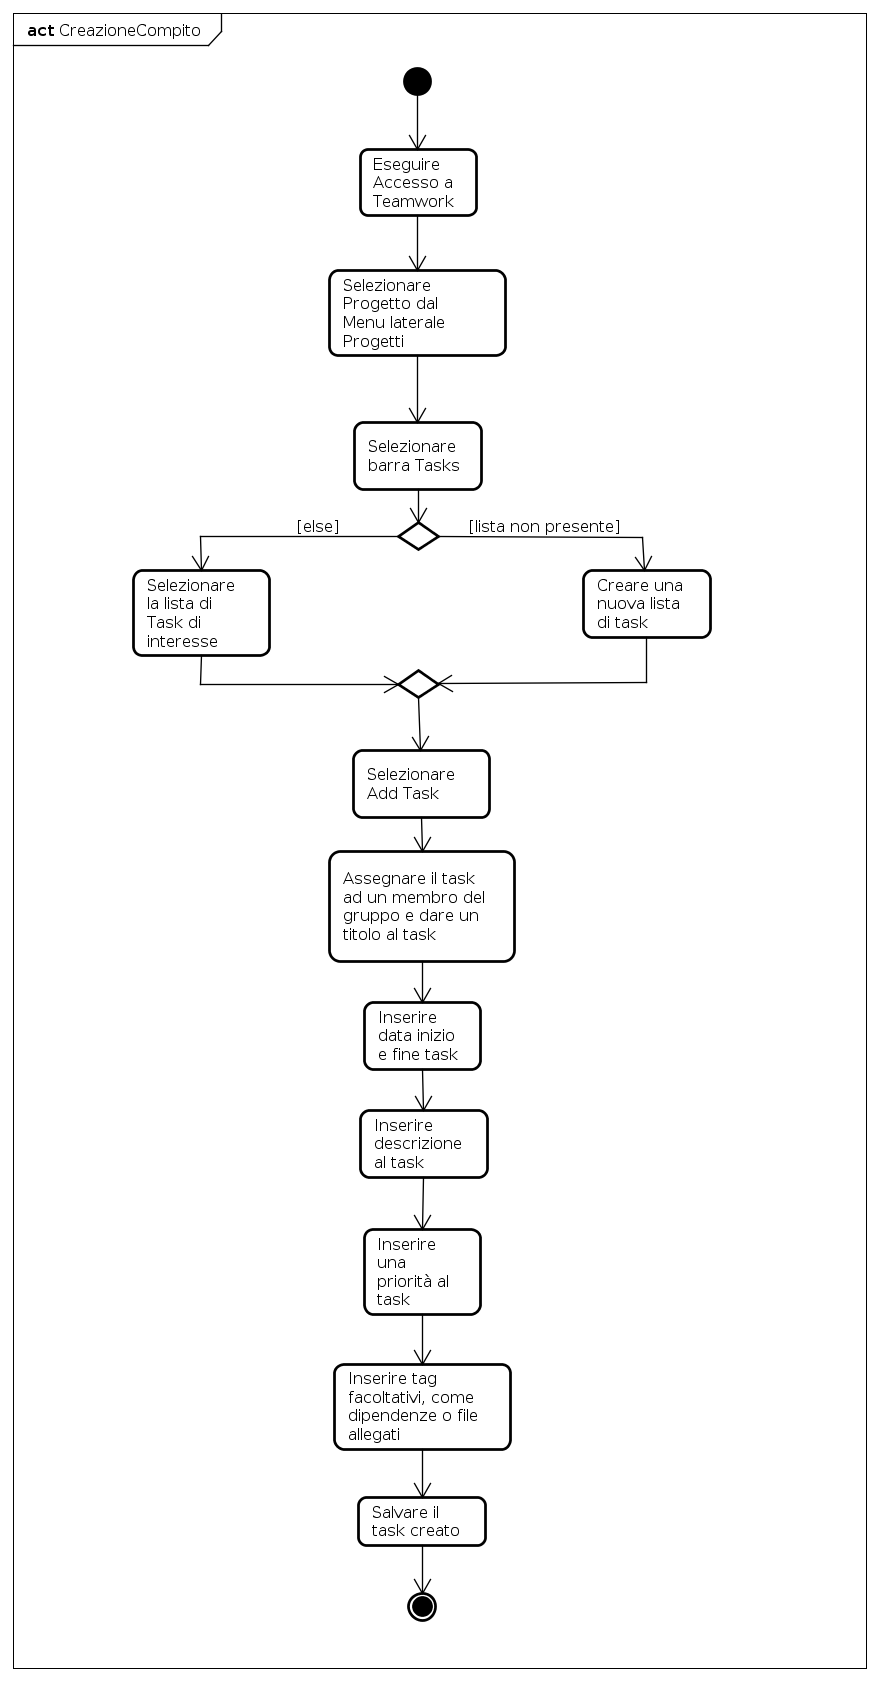
\includegraphics[width=10cm]{CreazioneCompito.png}
\caption{Diagramma attività - Creazione nuovo compito}
\end{figure}

\subsubsection{Modifica di un Compito}
L'operazione di modifica è molto semplice ed intuitiva. Viene descritta dal diagramma di attività che segue.
\begin{figure}[H]
\centering
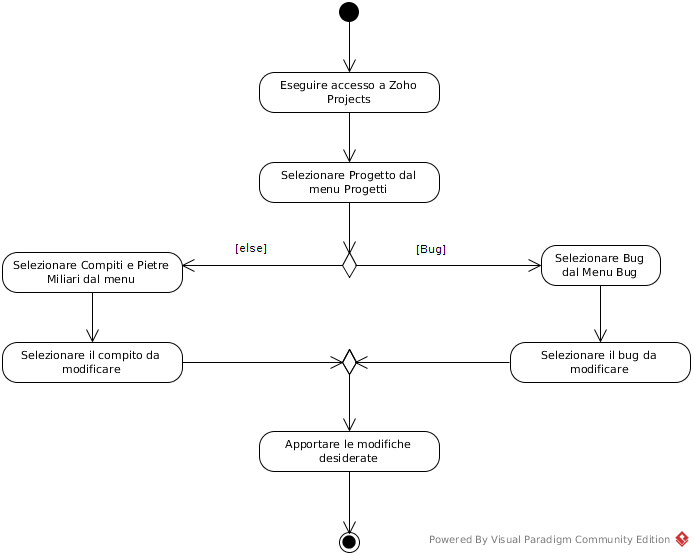
\includegraphics[width=10cm]{ModificaCompito.png}
\caption{Diagramma attività - Modifica Compito}
\end{figure}

\subsection{Strumenti per lo Sviluppo dell'Applicazione e per la Codifica}
\subsubsection{Framework}
Per realizzare il progetto si fa uso del \glossario{framework} \textbf{Play Framework}\footnote[5]{\url{https://www.playframework.com/}}. \\
\textbf{IntelliJ IDEA}\footnote[6]{\url{https://www.jetbrains.com/idea/}} è, invece, l'\glossario{IDE} utilizzato per lo sviluppo. La scelta è stata operata per una serie di motivi, tra cui l'ottima integrazione con lo strumento di versionamento, la pulita e semplice interfaccia grafica e gli strumenti per il \glossario{debugging}.
